\subsection{Análisis de la entropía}

Analizamos la entropía para las dos fuentes de información en cada uno de las experimentaciones.

En el caso de la red hogare\~na, para la experimentación sin intervención obtuvimos que la entropía es:
\begin{itemize}
\item $H_{Ssrc}$ = 1.9792698203575545
\item $H_{Sdst}$ = 3.7961238869546587
\end{itemize}

Comparando la entropía para cada fuente con la cantidad de información de los símbolos obtuvimos resultados que se aproximan a los esperados: una IP router más activa, con más probabilidad y por ende menos información. Decimos que se aproximan porque en el caso de los who-has enviados, el router efectivamente es el que tiene menos información, pero en el caso de los who-has recibidos, la IP del router y otras IPs tienen un valor muy similar.
En los siguientes histogramas se ve la cantidad de información para cada IP y la línea roja es la entropía, o sea la media:

\begin{figure}[!h]
	\begin{center}
		  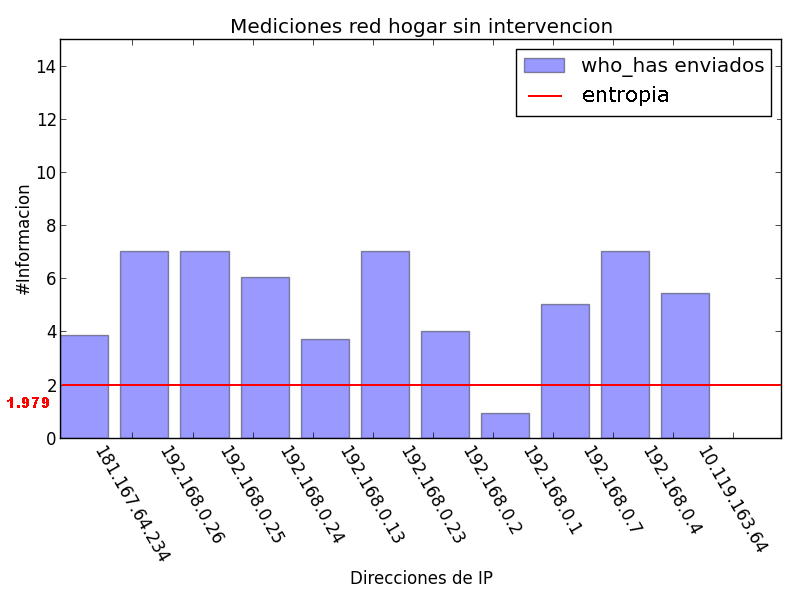
\includegraphics[scale=0.4]{Graficos/hogar_sin_sent_who_has.png}
		  \caption{Histograma red doméstica sin intervención, fuente: who-has enviados}
		  \label{fig:contra1}
	\end{center}
\end{figure}

\begin{figure}[!h]
	\begin{center}
		  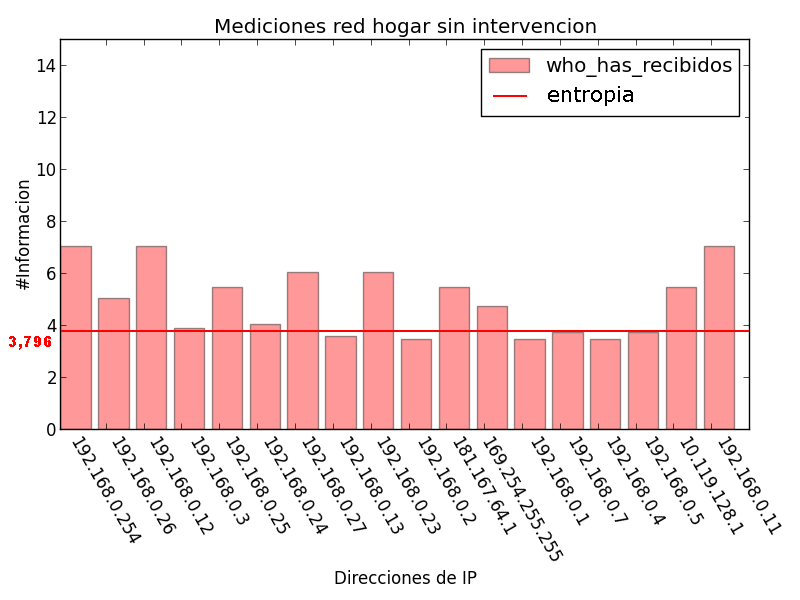
\includegraphics[scale=0.4]{Graficos/hogar_sin_received_who_has.png}
		  \caption{Histograma red doméstica sin intervención, fuente: who-has recibidos}
		  \label{fig:contra1}
	\end{center}
\end{figure}

Los nodos cuya cantidad de información está por debajo de la entropía son aquellos que son más activos y por ende tienen menos información.

En el caso de la red hogare\~na, para la experimentación con intervención obtuvimos los siguientes valores para la entropía de cada fuente:

\begin{itemize}
\item H(Ssrc) = 2.440087955604424
\item H(Sdst) = 2.9094618424425773
\end{itemize}

A diferencia de la experimentación anterior, hay nodos que emiten casi la misma cantidad de paquetes de tipo who-has que el router. Estos nodos son aquellos que en grafo direccionado, visto anteriormente, eran los nodos casi tan grandes como el router y que al perder conexión emiten un paquete ARP de tipo who-has. Por eso es que las cantidad emitida resulta próxima a la del router.
En cuanto a los paquetes de tipo who-has recibidos, el nodo que más paquetes recibe es el 169.254.255.255, que como explicamos antes, es la IP a la que se manda ARP cuando se pierde el servidor DHCP.

\begin{figure}[!h]
	\begin{center}
		  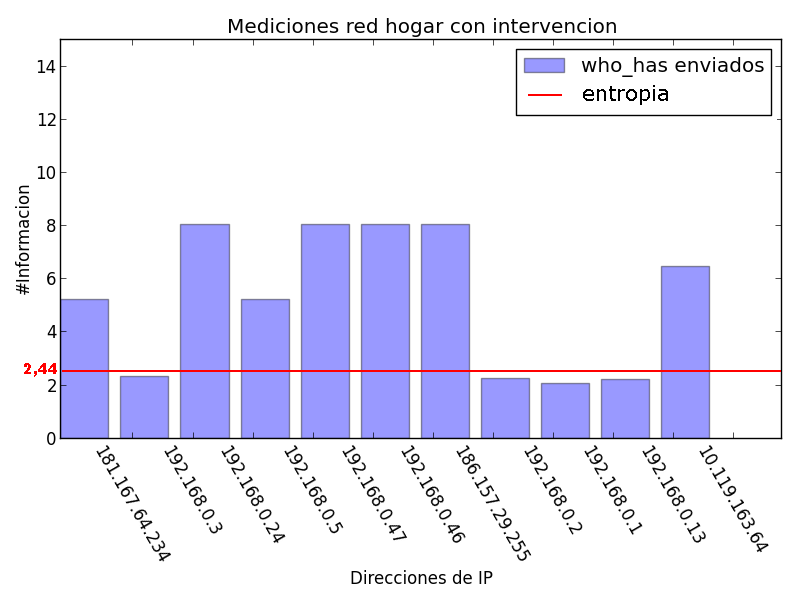
\includegraphics[scale=0.4]{Graficos/hogar_con_sent_who_has.png}
		  \caption{Histograma red doméstica con intervención, fuente: who-has enviados}
		  \label{fig:contra1}
	\end{center}
\end{figure}

\begin{figure}[!h]
	\begin{center}
		  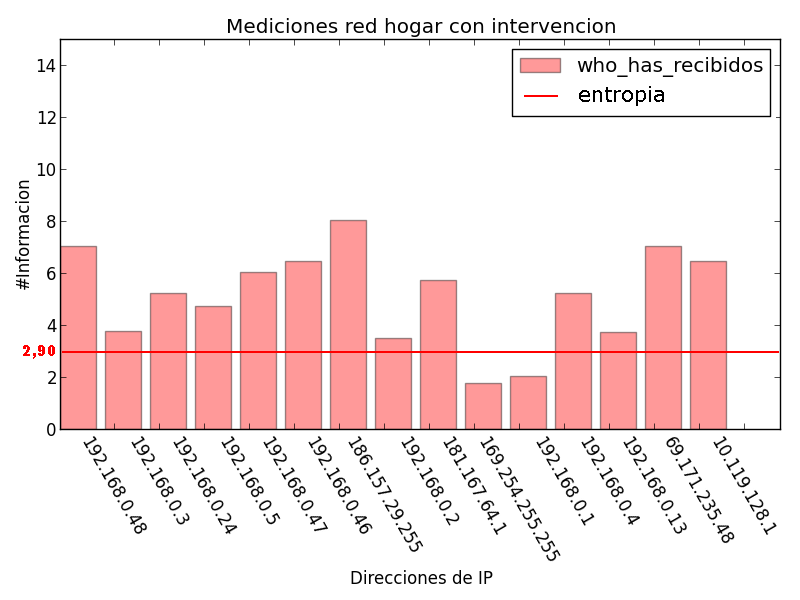
\includegraphics[scale=0.4]{Graficos/hogar_con_received_who_has.png}
		  \caption{Histograma red doméstica con intervención, fuente: who-has recibidos}
		  \label{fig:contra1}
	\end{center}
\end{figure}

En el caso de la red pública, obtuvimos los siguientes valores para la entropía de cada fuente:
\begin{itemize}
\item H(Ssrc) = 2.860373989857293
\item H(Sdst) = 1.7564032477264155
\end{itemize}

En esta experimentación el router es claramente el nodo que más paquetes who-has recibe. Pero en cuanto a los paquetes who-has emitidos, se ve que el router no es el que mas paquetes envía, sino que como se mencionó anteriormente hay 2 nodos(10.251.14.126 y 10.251.14.226) que son los principales emisores de paquetes ARP y que se mantuvieron muy activos a lo largo de la experimentación.

\begin{figure}[!h]
	\begin{center}
		  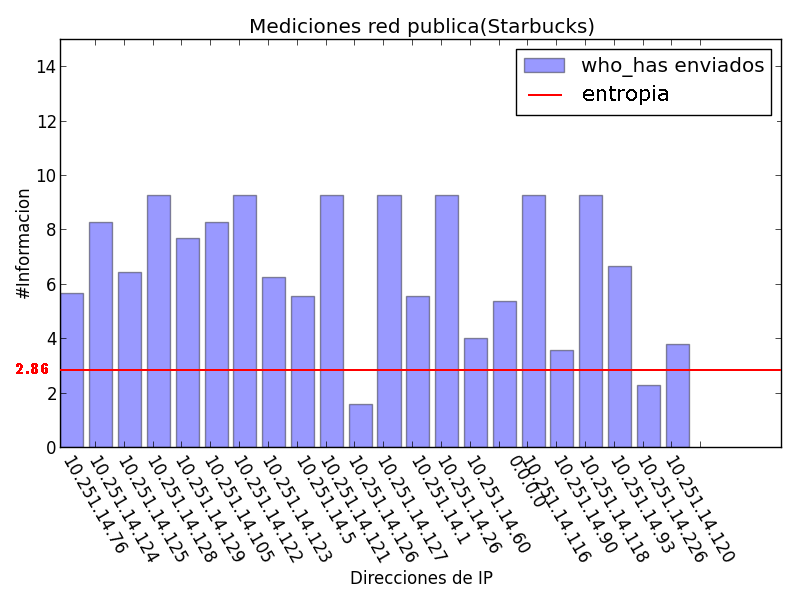
\includegraphics[scale=0.4]{Graficos/starbucks_sent_who_has.png}
		  \caption{Histograma Starbucks, fuente: who-has enviados}
		  \label{fig:contra1}
	\end{center}
\end{figure}

\begin{figure}[!h]
	\begin{center}
		  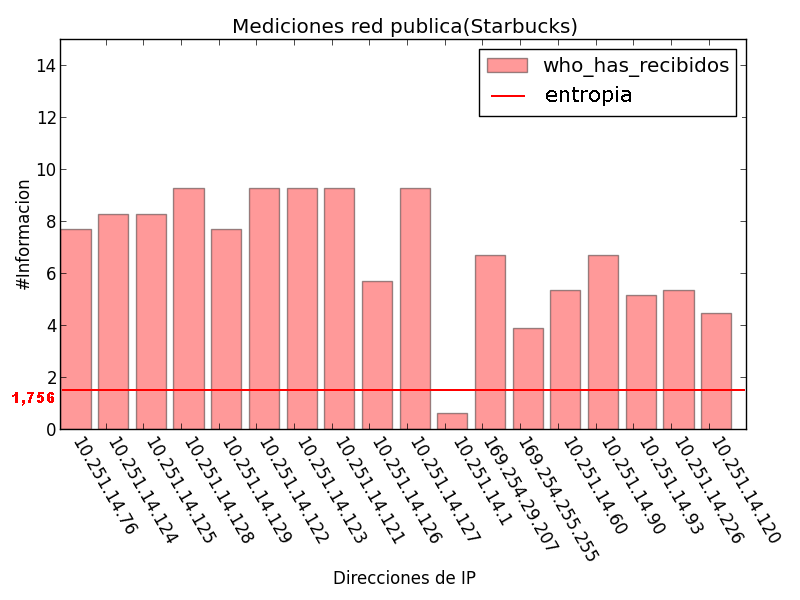
\includegraphics[scale=0.4]{Graficos/starbucks_received_who_has.png}
		  \caption{Histograma Starbucks, fuente: who-has recibidos}
		  \label{fig:contra1}
	\end{center}
\end{figure}



